\documentclass{jarticle}
\usepackage[dvipdfmx]{graphicx}
\usepackage{listings,jlisting,url,here}

\lstset{%
  language={C},
  basicstyle={\small},%
  identifierstyle={\small},%
  commentstyle={\small\itshape},%
  keywordstyle={\small\bfseries},%
  ndkeywordstyle={\small},%
  stringstyle={\small\ttfamily},
  frame={tb},
  breaklines=true,
  columns=[l]{fullflexible},%
  numbers=left,%
  xrightmargin=0zw,%
  xleftmargin=3zw,%
  numberstyle={\scriptsize},% stepnumber=1,
  numbersep=1zw,%
  lineskip=-0.5ex%
}
% xなんちゃらが変数,進捗書く
\newcommand{\xb}{催涙スプレーのゲージを表示}

% []内の数が引数,#数字で引数読む
\newcommand{\pitem}[1]{
  \item #1
}

\title{最終グループレポート}
\author{6119019207 矢野大暉}
\date{\number\year/\number\month/\number\day 提出}

\begin{document}
\maketitle

\section{ゲーム内容,操作方法(マニュアル)}
\subsection{ゲームのタイトル}
AGENT 3

\subsection{ジャンル}
脱出ゲーム

\subsection{概略}
ゲームの設定は,「犯罪組織に盗まれた金塊を組織に潜入して,複数のプレイヤーと協力して,組織的に取り返す」といった設定である.
本ゲームは,同一のサーバに接続した複数のプレイヤーが協力する脱出ゲームである.プレイヤーは出入り口からスタートし,敵(NPC),監視カメラに見からないように,ステージ上に設置された金塊をゲットし再び敵,監視カメラに見つからないように出入り口に帰ってくるゲームである.
ステージは全部で3つ用意されており,ステージが進むごとに難易度を向上させる.

プレイヤーは敵キャラや監視カメラに対して妨害を行うことで,他プレイヤーが金塊を取るためのアシストを行うことができる.
プレイヤーが行うことができる妨害として以下が挙げられる.
\begin{itemize}
\item 敵キャラに話しかける → 敵の視界の一時的な固定
\item 監視カメラのハッキング → 監視カメラが一時的に停止
\item 敵キャラに催涙スプレー → 敵の視界が一時的に無効化
\end{itemize}

\subsection{プレイ人数}
3人

\subsection{ルール}
ルールは以下のようになる.\\
1.	プレイヤー3人が入口から出発\\
2.	プレイヤーは,ステージに配置されている金塊を奪い返しに行く\\
3.	ステージに配置されている敵(NPC),監視カメラに見つからないように出口から脱出する\\

\subsection{遊び方}
以下の使用可能ツールを用いて,金塊を取り返し,出口からの脱出を試みる.\\\\
1.	催涙スプレー\\
敵の視界を奪い,動きを止めることができる\\
(右下の自分のゲージがなくなるまで使用可能)\\
2.	ハッキング\\
カメラの動きを止めることができる,各プレイヤーで1回のみ使用可能\\
(ゲージがたまるまでボタンを長押し,ゲージが溜まった状態で,ボタンを離した瞬間に3秒間カメラの首振りが停止する)\\
3.	会話\\
敵の視界が固定できる\\
各NPCに対して,計3回のみ使用可能\\



\subsection{操作方法}
本ゲームはゲームパッドでの操作を行う.

\begin{figure}[H]
\begin{center}
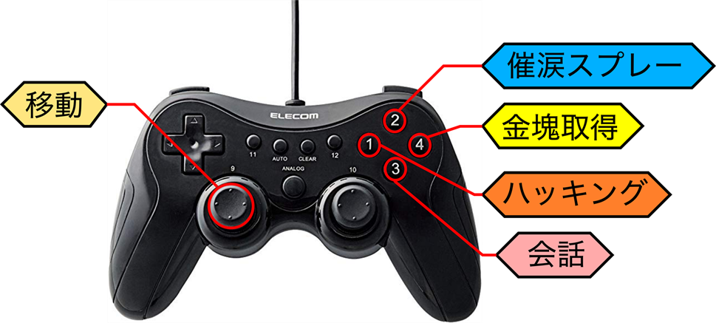
\includegraphics[width=\linewidth]{./zu/gamepad.png}
\caption{操作方法}
\label{fig:gamepad}
\end{center}
\end{figure}

\section{最終的なデータ構造,モジュール}
\subsection{サーバ,クライアント共通の変数,定数,構造体}

% map_height とかの定数を書く
\begin{table}[H]
  \begin{tabular}{|r|l|}
    \hline
    \multicolumn{2}{|l|}{ネットワーク関連の定数} \\ \hline
    DEFAULT\_PORT & デフォルトのポート番号51000 \\
    MAX\_LEN\_NAME  & クライアントのユーザ名の最大長 \\
    MAX\_NUM\_CLIENTS & 接続要求の受付最大数 \\
    MAX\_LEN\_BUFFER & メッセージの最大文字数 \\
    MAX\_LEN\_ADDR & 最大のアドレスの長さ \\
    BROADCAST & ブロードキャスト \\ \hline
  \end{tabular}
\end{table}
% サーバコマンドの定数はまた別に書く?
\begin{table}[H]
  \begin{tabular}{|r|l|}
    \hline
    \multicolumn{2}{|l|}{サーバーとクライアント間で送信されるコマンド} \\ \hline
    MESSAGE\_COMMAND & メッセージの送信\\
    ZAHYO\_COMMAND & 座標の送信\\
    KINKAI\_COMMAND & 金塊の状態\\
    HACK\_COMMAND & ハッキング状態\\
    HACK\_START\_COMMAND & ハッキング開始\\
    NOT\_HACK\_COMMAND & ハッキングキャンセル\\
    PLAYER\_COMMAND & プレイヤーが死んだことを示す\\
    UP\_COMMAND & 上へのスティック操作が行われたことを示す\\
    DOWN\_COMMAND & 下へのスティック操作が行われたことを示す\\
    RIGHT\_COMMAND & 右へのスティック操作が行われたことを示す\\
    LEFT\_COMMAND & 左へのスティック操作が行われたことを示す\\
    CENTER\_COMMAND &真ん中(左右)へのスティック操作が行われたことを示す\\
    AENTER\_COMMAND & 真ん中(上下)へのスティック操作が行われたことを示す\\
    X\_ON\_COMMAND & 2ボタンが押されたときに送信されるコマンド\\
    X\_OFF\_COMMAND & 2ボタンが離されたときに送信されるコマンド \\
    QUIT\_COMMAND & ゲームの終了\\
    START\_COMMAND & メニュー画面で,スタートボタンを押したことを表す\\
    ENEMY\_MODIFY\_COMMAND & 敵(NPC)の座標を同期する\\
    TALK\_START\_COMMAND & 会話を開始する\\
    TALK\_END\_COMMAND & 会話を終了する\\ \hline
  \end{tabular}
\end{table}

\begin{table}[H]
\begin{tabular}{|r|l|l|}
\hline
\multicolumn{3}{|l|}{CLIENT -- クライアントの構造体}       \\ \hline
データ型      & 変数名    & 内容        \\ \hline
int & cid & クライアントID \\
int  & sock     & ソケット番号  \\
sockaddr\_in & addr & IPアドレスやポート番号の情報  \\
  char[MAX\_LEN\_NAME] & name & 名前 \\ \hline
\end{tabular}
\end{table}


\begin{table}[H]
\begin{tabular}{|r|l|l|}
\hline
\multicolumn{3}{|l|}{CONTAINER -- コンテナの構造体}       \\ \hline
データ型      & 変数名    & 内容        \\ \hline
int & cid & クライアントID \\
  char & command & コマンド \\
  char[MAX\_LEN\_BUFFER] & message & メッセージ \\
  int & zahyo\_x & x座標 \\
  int & zahyo\_y & y座標 \\
  int[5] & enemy\_zahyo\_x  & 敵のx座標 \\
  int[5] & enemy\_zahyo\_y  & 敵のy座標 \\
  int[5] & move\_angle & 動く方向の角度 \\
  int[5] & prev\_angle & 現在向いている角度 \\\hline
\end{tabular}
\end{table}


\subsection{クライアントに必要な変数,構造体}
\begin{table}[H]
\begin{tabular}{|p{20em}|p{20em}|}
\hline
    定数名  & 内容\\ \hline
    WINDOWWIDTH & ウィンドウの幅 \\ 
    WINDOWHEIGHT & ウィンドウの高さ \\
    PLAYER\_NUM & プレイヤーの数 \\
    PLAYER\_SPEED & プレイヤーのスピード \\
    CAMERA\_NUM & 監視カメラの数 \\
    BACKGROUND\_NUM & 背景画像の数 \\
    FONT\_NUM & システムメッセージの数 \\
    ENEMY\_SPEED & 敵(NPC)のスピード \\
    KOTEI\_OBJECT\_NUM\_MAX & マップに読み込めるオブジェクトの最大の数 \\
    MAP\_CHIPSIZE & マップの1オブジェクトの大きさ \\
    MAP\_WIDTH & 横にマップのオブジェクトがいくつ置けるか \\
    MAP\_HEIGHT & 縦にマップのオブジェクトをいくつ置けるか \\
    SPRAY\_WIDTH & 催涙スプレーの幅 \\
    SPRAY\_HEIGHT & 催涙スプレーの高さ \\
    SAIRUI\_TIME & 催涙スプレーで止まる時間 \\
    SPRAY\_TIME & 催涙スプレーが使える時間 \\
    TALK\_TIME & 会話時間 \\
    TALK\_NUM & 敵(NPC)に何回まで話せるか \\
    HACKTIME & ハッキングに要する時間 \\
    STOPTIME & ハッキング中に,カメラを止める時間 \\
    MENUMODE, GAMEMODE, RESULTMODE, STAGENUMMODE & ゲーム中のモード番号 \\
    ENEMY\_NUM & 敵(NPC)の数\\ \hline
\end{tabular}
\end{table}



\begin{table}[H]
\begin{tabular}{|p{13em}|p{13em}|p{12em}|}
    \hline
    データ型 & 変数名 & 内容 \\ \hline
    const int & fps & 1秒間に何回画面を描画するか \\
    const int & framedelay & 1回の描画にかけるべき時間 \\
    Uint32 & framestart & フレーム処理の始まりの時間を格納する変数 \\
    Uint32 & modi\_before & プレイヤーの座標を修正するのに使う時間 \\
    int & frametime & 1回の処理にかかった時間を格納する \\
    int & modi\_time & 座標更新の間隔の時間 \\
    u\_short & port & ポート番号 \\
    char & server\_name & サーバー名 \\
    TTF\_Font* & japanesefont & ゲーム内フォント \\
    bool & up &  メニュー画面の上を選択していることを判別するフラグ \\
    bool & down &メニュー画面の下を選択していることを判別するフラグ\\
    bool & kinkai\_flag & 金塊描画フラグ \\
    bool & hacking\_flag & ハッキング処理フラグ \\
    bool & player\_flag & プレイヤー描画のフラグ\\
    int & before\_enemy\_x & 敵の以前のx座標 \\
    int & before\_enemy\_y & 敵の以前のy座標 \\
    Uint32 & random\_start & ランダム移動を開始した時間を格納する変数 \\  
    int & time\_now & ハッキング時間を判定するときに判別する変数 \\
    float & gauge & ハッキングの際に描画されるゲージ \\
    int[15][20] & map0,map1,map2 & ゲームのマップの変数 \\
    static char *[TYPE\_NUM] & imgfiles & 読み込む画像ファイル \\
    static char *[FONT\_NUM] & fonts & システムメッセージの内容 \\
    static char *[2]& text\_fukidashi & 会話コマンドでフキダシの中に描画される内容 \\
    static SDL\_Rect & camera\_dst\_rects & ステージごとのカメラの座標\\ 
    static int [ENEMY\_NUM] & enemy\_moveangles & 敵(NPC)が最初に向いている方向 \\
    static enemymovetype [ENEMY\_NUM] & enemy\_movetypes & 敵(NPC)の動きのパターン \\ 
    static SDL\_Rect [FONT\_NUM] & font\_dst\_rects & メッセージが描画される座標 \\
    int & kotei\_object\_num & 1マップのオブジェクトの数 \\
    int[ENEMY\_NUM] & savestopenemy & 動かないタイプの敵(NPC)が何番目かを格納する変数\\
    int & lrflag & 敵の視界が左回りか右回りかを分けるフラグ \\ \hline
  \end{tabular}
\end{table}

\begin{table}[H]
\begin{tabular}{|p{13em}|p{13em}|p{12em}|}
    \hline
    データ型 & 変数名 & 内容 \\ \hline
    int & status & ゲームの現在の状態 \\
    bool & run & ゲームが動作中かどうか \\
    bool[ENEMY\_NUM] & same\_place\_flag & 敵(NPC)が一定時間同じ座標にとどまっているかどうかを示すフラグ \\
    bool[ENEMY\_NUM] & random\_start\_flag & 敵(NPC)が一定時間同じ座標にとどまったため,ランダムウォークを始めたことを示すフラグ \\
    Uint32[ENEMY\_NUM] & stay\_start & 敵(NPC)がとどまっている時間を格納する変数 \\ 
    int[ENEMY\_NUM] & stay\_time & 敵(NPC)がランダムウォークをする時間を格納する変数\\
    int & myid & 自分自身のクライアントIDを示す変数 \\
    int & stage\_num & ステージの通し番号 \\
    bool & stage\_trans\_flag & ステージ遷移するか判別するフラグ \\
    bool & game\_over\_flag & ゲームオーバーかどうか判別するフラグ \\ \hline
  \end{tabular}
\end{table}

\begin{table}[H]
\begin{tabular}{|r|l|l|}
\hline
\multicolumn{3}{|l|}{objectinfo -- 画面に表示するオブジェクト(壁,敵など)情報の構造体}       \\ \hline
データ型      & 変数名    & 内容        \\ \hline
objecttype    & type & オブジェクトの種類  \\
SDL\_Texture* & image\_texture     & オブジェクトのテクスチャ \\
SDL\_Rect & src\_rect & 元画像を読み取る領域 \\
SDL\_Rect & dst\_rect & 画像の出力先の領域 \\ \hline
\end{tabular}
\end{table}


\begin{table}[H]
\begin{tabular}{|l|l|}
\hline
  \multicolumn{2}{|l|}{objectinfo -- オブジェクトタイプを示す定数 }\\ \hline
定数名    & 内容        \\ \hline
  TYPE\_NONE & なにもないことを表す \\
  TYPE\_KINKAI & 金塊を表す \\
  TYPE\_SHELF & 棚を表す \\
  TYPE\_CAMERA & カメラを表す \\
  TYPE\_ENTRANCE & 出入口を表す \\
  TYPE\_ENEMY & 敵(NPC)を表す  \\
  TYPE\_PLAYER1& プレイヤー1を表す \\
  TYPE\_PLAYER2 &プレイヤー2を表す \\
  TYPE\_PLAYER&プレイヤー3を表す \\
  TYPE\_ENEMY\_MOVING\_FLOOR\_UL & 移動床1を表す  \\
  TYPE\_ENEMY\_MOVING\_FLOOR\_UR &移動床1を表す  \\
  TYPE\_ENEMY\_MOVING\_FLOOR\_DL &移動床1を表す  \\
  TYPE\_ENEMY\_MOVING\_FLOOR\_DR &移動床1を表す  \\
  TYPE\_ENEMY\_MOVING\_FLOOR\_REV &移動床1を表す  \\
  TYPE\_BACKGROUND & 背景を表す \\
  TYPE\_SPRAY & 催涙スプレーを表す \\
  TYPE\_NUM& タイプの総数を表す \\ \hline
\end{tabular}
\end{table}


\begin{table}[H]
\begin{tabular}{|r|l|l|}
\hline
\multicolumn{3}{|l|}{inputkeys -- ジョイパッドからの入力を保存する構造体}       \\ \hline
データ型      & 変数名    & 内容        \\ \hline
Uint32    & left,right,up,down & アナログスティックの入力方法を保存する \\
Uint32    & a,x,y,b & ボタンの入力方法を保存する \\ \hline
\end{tabular}
\end{table}

\begin{table}[H]
\begin{tabular}{|r|l|p{25em}|}
\hline
\multicolumn{3}{|l|}{プレイヤーの構造体}       \\ \hline
データ型      & 変数名    & 内容        \\ \hline
objecttype    & type & オブジェクトの種類  \\
SDL\_Texture* & image\_texture     & プレイヤーのテクスチャ \\
SDL\_Texture* & spray\_texture     & 催涙スプレーのテクスチャ \\
SDL\_Rect & src\_rect & 元画像を読み取る領域 \\
SDL\_Rect & dst\_rect & 画像の出力先の領域 \\
float & back\_zahyo\_x & 小数で表されたプレイヤーの正確なx座標\\
float & back\_zahyo\_y & 小数で表されたプレイヤーの正確なy座標\\
bool & flag\_kinkai & プレイヤーが金塊を取得したか判別するフラグ\\
bool & flag\_hack\_start & ハッキングを開始フラグ\\
bool & flag\_hack\_end & ハッキングを終了フラグ\\
int &hack & ハッキングできる回数\\
int & inputtime & ハッキング開始した時間を保存する\\
int & speed & プレイヤーの速度\\
inputkeys &key & 入力されたキー情報を保存\\
int & look\_angle & プレイヤーが向いている角度\\
int & spray\_flag & スプレーを出しているか判別するフラグ\\
SDL\_Rect & spray\_src\_rect & 催涙スプレーテクスチャを読み取る範囲\\
SDL\_Rect & spray\_dst\_rect & 催涙スプレーテクスチャを出力する範囲\\
int[2][4] & spray\_hitline & 催涙スプレーの当たり判定\\
SDL\_Point &spray\_origin &  催涙スプレーが出てくる座標 \\
int & spraytime & 催涙スプレーが使える残り時間\\
int & talkstarttime & 会話を開始した時間\\
bool & flag\_talk & 会話をしているか判別するフラグ \\
bool & flag\_fukidasiflip & 位置によって会話の際のフキダシを反転する必要があるか判定するフラグ\\ \hline
\end{tabular}
\end{table}

\begin{table}[H]
\begin{tabular}{|r|l|l|}
\hline
\multicolumn{3}{|l|}{camerainfo -- カメラ情報の構造体}       \\ \hline
データ型      & 変数名    & 内容        \\ \hline
SDL\_Texture* & image\_texture     & カメラのテクスチャ \\
SDL\_Rect & src\_rect & 元画像を読み取る領域 \\
SDL\_Rect & dst\_rect & 画像の出力先の領域 \\
bool & flag\_kinkai& 金塊を持っているか判別するフラグ\\
bool & flag\_hack & ハッキングをしているか判別するフラグ\\
int[2][3] & tri & カメラ視界の当たり判定の三角形\\
float[3] &  theta & カメラの角度 \\
clockwise & bool & カメラの回転方向を指定する\\
double & angle & カメラの向いている方向\\ \hline
\end{tabular}
\end{table}

\begin{table}[H]
\begin{tabular}{|r|l|l|}
\hline
\multicolumn{3}{|l|}{enemyinfo -- 敵(NPC)の構造体}       \\ \hline
データ型      & 変数名    & 内容        \\ \hline
objecttype    & type & オブジェクトの種類  \\
SDL\_Texture* & image\_texture     & 敵(NPC)のテクスチャ \\
SDL\_Rect & src\_rect & 元画像を読み取る領域 \\
SDL\_Rect & dst\_rect & 画像の出力先の領域 \\
 SDL\_Rect & prev\_overlap\_rect & 一時的にオブジェクトと重なった範囲を保存する\\
bool & flag\_kinkai & 金塊を取ったかどうか判別するフラグ \\
bool & speed & 敵(NPC)の移動速度\\
int & move\_angle & 敵が動く方向\\
bool & flag\_sairui & 催涙スプレーを食らっているか判別するフラグ \\
enemymovetype  & movetype & 敵の動きのタイプ \\
unsigned int  & savetime & 催涙スプレーを食らった時間を保存する \\
int[2][3] & tri & 敵(NPC)視界の当たり判定の三角形 \\
int & prev\_angle & 現在敵(NPC)が向いている角度 \\
int  & talk\_angle & プレイヤーが会話してきたときの角度 \\
bool & flag\_talk & 会話しているか判別するフラグ \\
int & talkstarttime & 会話の開始時間 \\
bool & flag\_one\_talk & 会話を一回したか判別するフラグ \\
int & talktime & 会話時間 \\
int & talknum & これまでに会話した回数を保存\\
bool & flag\_fukidasiflip & フキダシを反転するか判別するフラグ \\ \hline
\end{tabular}
\end{table}

\begin{table}[H]
\begin{tabular}{|r|l|l|}
\hline
\multicolumn{3}{|l|}{backgroundinfo -- 背景の構造体}       \\ \hline
データ型      & 変数名    & 内容        \\ \hline
SDL\_Texture* & image\_texture     & 背景のテクスチャ \\
SDL\_Rect & src\_rect & 元画像を読み取る領域 \\
SDL\_Rect & dst\_rect & 画像の出力先の領域 \\ \hline
\end{tabular}
\end{table}

\begin{table}[H]
\begin{tabular}{|r|l|l|}
\hline
\multicolumn{3}{|l|}{fontinfo -- フォントの構造体}       \\ \hline
データ型      & 変数名    & 内容        \\ \hline
SDL\_Texture* & image\_texture     & フォントのテクスチャ \\
SDL\_Rect & src\_rect & 元画像を読み取る領域 \\
SDL\_Rect & dst\_rect & 画像の出力先の領域 \\ \hline
\end{tabular}
\end{table}

\begin{table}[H]
\begin{tabular}{|r|l|l|}
\hline
\multicolumn{3}{|l|}{fukidashiinfo-- フキダシの構造体}       \\ \hline
データ型      & 変数名    & 内容        \\ \hline
SDL\_Texture* & image\_texture     & フキダシのテクスチャ \\
SDL\_Rect & src\_rect & 元画像を読み取る領域 \\
SDL\_Rect & dst\_rect & 画像の出力先の領域 \\
SDL\_Texture*[2] & textimage & 会話時のテキスト内容 \\
SDL\_Rect & font\_src\_rect & フォントの元を読み取る領域 \\ \hline
\end{tabular}
\end{table}

\subsection{クライアントで使用するモジュール}
\begin{table}[H]
\begin{tabular}{|r|l|}
\hline
\multicolumn{2}{|l|}{void Startup(void)}       \\ \hline
関数名           & Startup \\ \hline
機能     & ゲームの初期化を行う関数 \\
引数     & なし \\
返り値   & なし \\ \hline
\end{tabular}
\end{table}


\begin{table}[H]
\begin{tabular}{|r|l|}
\hline
\multicolumn{2}{|l|}{void SetCamera(void)}       \\ \hline
関数名           & SetCamera \\ \hline
機能     & カメラの初期値を設定する関数 \\
引数     & なし \\
返り値   & なし \\ \hline
\end{tabular}
\end{table}

\begin{table}[H]
\begin{tabular}{|r|l|}
\hline
\multicolumn{2}{|l|}{void Fontload(void)}       \\ \hline
関数名           & Fontload \\ \hline
機能     & フォントの読み込みを行う関数 \\
引数     & なし \\
返り値   & なし \\ \hline
\end{tabular}
\end{table}

\begin{table}[H]
\begin{tabular}{|r|l|}
\hline
\multicolumn{2}{|l|}{void Imageload(void)}       \\ \hline
関数名   & Imageload \\ \hline
機能     & 背景,カメラ画像の読み込みを行う関数 \\
引数     & なし \\
返り値   & なし \\ \hline
\end{tabular}
\end{table}



\begin{table}[H]
\begin{tabular}{|r|l|}
\hline
\multicolumn{2}{|l|}{void MakeMap(void)}       \\ \hline
関数名   & MakeMap \\ \hline
機能     & マップの読み込みと配置を行う関数 \\
引数     & なし \\
返り値   & なし \\ \hline
\end{tabular}
\end{table}

\begin{table}[H]
\begin{tabular}{|r|l|}
\hline
\multicolumn{2}{|l|}{void InitObjectFromMap(void)}       \\ \hline
関数名   & InitObjectFromMap \\ \hline
機能     & マップ変数からオブジェクトの配置と初期化を行う \\
引数     & なし \\
返り値   & なし \\ \hline
\end{tabular}
\end{table}



\begin{table}[H]
\begin{tabular}{|r|l|}
\hline
\multicolumn{2}{|l|}{void setup\_client(cahr *server\_name ,u\_short port)}       \\ \hline
関数名           & setup\_client \\ \hline
機能     & クライアントのセットアップを行う関数 \\
引数     & なし \\
返り値   & なし \\ \hline
\end{tabular}
\end{table}

\begin{table}[H]
\begin{tabular}{|r|l|}
\hline
  \multicolumn{2}{|l|}{void send\_data(void *data, int size}       \\ \hline
関数名           & send\_data \\ \hline
機能     & サーバにデータを送信する関数 \\
引数     & なし \\
返り値   & なし \\ \hline
\end{tabular}
\end{table}



\begin{table}[H]
\begin{tabular}{|r|l|}
\hline
\multicolumn{2}{|l|}{void Input(void)}  \\ \hline
関数名           & Input \\ \hline
機能     & ジョイパッドの入力を読み取る関数 \\
引数     & なし \\
返り値   & なし \\ \hline
\end{tabular}
\end{table}

\begin{table}[H]
\begin{tabular}{|r|l|}
\hline
\multicolumn{2}{|l|}{int control\_requests(void)}       \\ \hline
関数名           & control\_requests \\ \hline
機能     & サーバからのデータを受信し,データに応じた処理をする関数 \\
引数     & なし \\
返り値   & 0 or 1 \\ \hline
\end{tabular}
\end{table}


\begin{table}[H]
\begin{tabular}{|r|l|}
\hline
\multicolumn{2}{|l|}{int execute\_command(void)}       \\ \hline
関数名           & execute\_command \\ \hline
機能     & サーバから送られてきたコマンドを実行する \\
引数     & なし \\
返り値   & 0 or 1 \\ \hline
\end{tabular}
\end{table}


\begin{table}[H]
\begin{tabular}{|r|l|}
\hline
\multicolumn{2}{|l|}{void receive\_data(void *data, int size)}       \\ \hline
関数名   & receive\_data \\ \hline
機能     & サーバからのデータを受け取る関数 \\
引数     & なし \\
返り値   & なし \\ \hline
\end{tabular}
\end{table}


\begin{table}[H]
\begin{tabular}{|r|l|}
\hline
\multicolumn{2}{|l|}{void Stage\_Renew(void)}       \\ \hline
関数名           & Stage\_Renew \\ \hline
機能     & ステージ遷移する際にステージの初期化をする関数 \\
引数     & なし \\
返り値   & なし \\ \hline
\end{tabular}
\end{table}

\begin{table}[H]
\begin{tabular}{|r|l|}
\hline
\multicolumn{2}{|l|}{void DrawMenu(void)}       \\ \hline
関数名           & DrawMenu \\ \hline
機能     & メニュー画面を描画する \\
引数     & なし \\
返り値   & なし \\ \hline
\end{tabular}
\end{table}


\begin{table}[H]
\begin{tabular}{|r|l|}
\hline
\multicolumn{2}{|l|}{void MoveChara(void)}       \\ \hline
  関数名           & MoveChara \\ \hline
機能     & キャラクター(敵,プレイヤーなど)を動かす関数 \\
引数     & なし \\
返り値   & なし \\ \hline
\end{tabular}
\end{table}


\begin{table}[H]
\begin{tabular}{|r|l|}
\hline
\multicolumn{2}{|l|}{void PlayerAction(void)}       \\ \hline
関数名           & PlayerAction \\ \hline
機能     & 催涙スプレー,会話処理を行う関数 \\
引数     & なし \\
返り値   & なし \\ \hline
\end{tabular}
\end{table}


\begin{table}[H]
\begin{tabular}{|r|l|}
\hline
\multicolumn{2}{|l|}{void ChangeEnemyMoveAngle(void)}       \\ \hline
関数名           & ChangeEnemyMoveAngle \\ \hline
  機能     & 敵(NPC)があるオブジェクトに重なったときに特定の方向へ動く方向を変える関数 \\
引数     & なし \\
返り値   & なし \\ \hline
\end{tabular}
\end{table}


\begin{table}[H]
\begin{tabular}{|r|l|}
\hline
\multicolumn{2}{|l|}{void MoveTriangle(void)}       \\ \hline
関数名           & MoveTriangle \\ \hline
機能     & カメラ,敵の視界の三角形を動かす \\
引数     & なし \\
返り値   & なし \\ \hline
\end{tabular}
\end{table}


\begin{table}[H]
\begin{tabular}{|r|l|}
\hline
\multicolumn{2}{|l|}{float Rotation(int x1, int y1, int a, int b, double theta, int *x2, int *y2)}       \\ \hline
関数名           & Rotation \\ \hline
機能     & xとyと角度を引数に与えて回転後の座標を返す関数 \\
引数     & x座標,y座標,角度 \\
返り値   & 回転後の座標 \\ \hline
\end{tabular}
\end{table}


\begin{table}[H]
\begin{tabular}{|r|l|}
\hline
\multicolumn{2}{|l|}{void Collision(void)}       \\ \hline
関数名           & Collision \\ \hline
  機能     & カメラ,敵(NPC)との衝突を検知する関数 \\
引数     & なし \\
返り値   & なし \\ \hline
\end{tabular}
\end{table}


\begin{table}[H]
\begin{tabular}{|r|l|}
\hline
\multicolumn{2}{|l|}{void RenderWindow(void)}       \\ \hline
関数名           & RenderWindow \\ \hline
機能     & 画面の描画を行う関数 \\
引数     & なし \\
返り値   & なし \\ \hline
\end{tabular}
\end{table}


\begin{table}[H]
\begin{tabular}{|r|l|}
\hline
\multicolumn{2}{|l|}{void Events(void)} \\ \hline
関数名           & Events \\ \hline
  機能     & ハッキングを行う関数 \\
引数     & なし \\
返り値   & なし \\ \hline
\end{tabular}
\end{table}


\begin{table}[H]
\begin{tabular}{|r|l|}
\hline
\multicolumn{2}{|l|}{void StageNumShow(void)}       \\ \hline
関数名           & StageNumShow \\ \hline
機能     & ステージに応じた表示をする関数 \\
引数     & なし \\
返り値   & なし \\ \hline
\end{tabular}
\end{table}

\begin{table}[H]
\begin{tabular}{|r|l|}
\hline
\multicolumn{2}{|l|}{void terminate\_client(void)}       \\ \hline
関数名           & terminate\_client \\ \hline
機能     & ソケットの切断を行う関数 \\
引数     & なし \\
返り値   & なし \\ \hline
\end{tabular}
\end{table}


\begin{table}[H]
\begin{tabular}{|r|l|}
\hline
\multicolumn{2}{|l|}{void joystick\_send(int num)}       \\ \hline
関数名           & joystick\_send \\ \hline
機能     & ジョイスティックの操作に関する情報を送信する関数 \\
引数     & コマンド番号 \\
返り値   & なし \\ \hline
\end{tabular}
\end{table}


\begin{table}[H]
\begin{tabular}{|r|l|}
\hline
\multicolumn{2}{|l|}{void handle\_error(void)}       \\ \hline
関数名           & handle\_error \\ \hline
機能     & エラーメッセージを出力する関数 \\
引数     & なし \\
返り値   & なし \\ \hline
\end{tabular}
\end{table}

\begin{table}[H]
\begin{tabular}{|r|l|}
\hline
  \multicolumn{2}{|l|}{void Destroy(void)}       \\ \hline
関数名           & Destroy \\ \hline
機能     & ゲームを終了する関数 \\
引数     & なし \\
返り値   & なし \\ \hline
\end{tabular}
\end{table}


\subsection{サーバに必要な変数,構造体}
\begin{table}[H]
  \begin{tabular}{|r|l|l|}
    \hline
    データ型 & 変数名 & 内容 \\ \hline
    int & num\_clients& クライアント数 \\
    int & num\_socks & ソケット数 \\
    fd\_set & mask;  &FD集合を表す構造体 \\
    int & start\_count & スタートカウント \\
    int[3] & start\_count\_flag & クライアント3台の同期をとるためのフラグ \\ \hline
\end{tabular}
\end{table}

\subsection{サーバで使用するモジュール}

\begin{table}[H]
\begin{tabular}{|r|l|}
\hline
  \multicolumn{2}{|l|}{void setup\_server(int num\_cl, u\_short port)}       \\ \hline
関数名           & setup\_server \\ \hline
機能     & サーバーのセットアップを行う関数 \\
引数     & クライアント数, ポート番号 \\
返り値   & なし \\ \hline
\end{tabular}
\end{table}


\begin{table}[H]
\begin{tabular}{|r|l|}
\hline
  \multicolumn{2}{|l|}{int control\_request(void)}       \\ \hline
関数名           & control\_request \\ \hline
機能     & クライアントからのデータを受信し,データに応じた処理をする関数 \\
引数     & なし \\
返り値   & 1のとき処理を続け,0のとき処理を終了する. \\ \hline
\end{tabular}
\end{table}


\begin{table}[H]
\begin{tabular}{|r|l|}
\hline
  \multicolumn{2}{|l|}{void terminate\_server(void)}       \\ \hline
関数名           & terminate\_server \\ \hline
機能     & サーバを終了する処理 \\
引数     & なし \\
返り値   & なし \\ \hline
\end{tabular}
\end{table}


\begin{table}[H]
\begin{tabular}{|r|l|}
\hline
  \multicolumn{2}{|l|}{void send\_data(int cid, void *data, int size)}       \\ \hline
関数名           & send\_data \\ \hline
機能     & クライアントにデータを送信する関数 \\
引数     & クライアントID, データ, データサイズ \\
返り値   & なし \\ \hline
\end{tabular}
\end{table}

\begin{table}[H]
\begin{tabular}{|r|l|}
\hline
  \multicolumn{2}{|l|}{void receive\_data(int cid, void *data, int size)}       \\ \hline
関数名           & send\_data \\ \hline
機能     & クライアントからデータを受信する関数 \\
引数     & クライアントID, データ, データサイズ \\
返り値   & なし \\ \hline
\end{tabular}
\end{table}

\begin{table}[H]
\begin{tabular}{|r|l|}
\hline
\multicolumn{2}{|l|}{void handle\_error(void)}       \\ \hline
関数名           & handle\_error \\ \hline
機能     & エラーメッセージを出力する関数 \\
引数     & なし \\
返り値   & なし \\ \hline
\end{tabular}
\end{table}


\section{ファイルの構成,プログラムの起動方法,注意点}
common.h クライアントで使用するヘッダファイル \\
 constants.h サーバ,クライアントで使用するヘッダファイル \\
 \\
─source クライアント側のファイルをまとめたフォルダ \\
  │  agent クライアントの実行ファイル \\
  │  fonts-japanese-gothic.ttf 日本語のフォントファイル \\
  │  func.c クライアントで使用する関数をまとめたファイル \\
  │  func.h func.cで使用するヘッダファイル \\
  │  main.c クライアントのメインプログラム \\
  │  Makefile クライアントのmakeファイル \\
  │ \\
  ├─bgm ゲーム内で使用するBGM \\
  │      bgm1.mp3 \\
  │ \\
  └─images ゲーム内で使用する画像素材 \\
\hspace{3em}    bg.png \\
\hspace{3em}    camera.png \\
\hspace{3em}    enemy.png \\
\hspace{3em}    entrance.png \\
\hspace{3em}    floor.png \\
\hspace{3em}    floor\_dl.png \\
\hspace{3em}    floor\_dr.png \\
\hspace{3em}    floor\_rev.png \\
\hspace{3em}    floor\_ul.png \\
\hspace{3em}    floor\_ur.png \\
\hspace{3em}    fukidasi.png \\
\hspace{3em}    fukidasi.xcf \\
\hspace{3em}    kinkai.png \\
\hspace{3em}    menu.png \\
\hspace{3em}    player.png \\
\hspace{3em}    player1\_8pattern.png \\
\hspace{3em}    player1\_8pattern.xcf \\
\hspace{3em}    player2.png \\
\hspace{3em}    player2\_8pattern.png \\
\hspace{3em}    player2\_8pattern.xcf \\
\hspace{3em}    player3.png \\
\hspace{3em}    player3\_8pattern.png \\
\hspace{3em}    player3\_8pattern.xcf \\
\hspace{3em}    shelf.png \\
\hspace{3em}    spray.png \\
 \\
─source\_server サーバ側のファイルをまとめたフォルダ \\
\hspace{3em}       main.c サーバのメインプログラム \\
 \hspace{3em}      main.o \\
 \hspace{3em}      Makefile サーバのmakeファイル \\
 \hspace{3em}      server サーバの実行ファイル \\
 \hspace{3em}      server.c サーバで使用する関数をまとめたファイル \\
 \hspace{3em}      server.o \\

\subsection{プログラムの起動,終了方法}
\subsubsection{起動方法}
1.プレイヤー3人のうちの誰かがサーバを起動する.\\
./server 3

2.各プレイヤーがサーバに繋げる \\
./agent clpc108

\subsubsection{終了方法}
ゲームパッドの12番ボタンを押す.


\section{班としての反省点} %完成
ゲームの作り込みを優先するあまり,ゲームの基礎部分がおろそかになってしまい実装が遅れた点.
プレイヤーを追跡するNPCの動きやプレイヤーの妨害アクションの実装にこだわり,ステージ遷移とゲーム終了処理の実装を後にまわしてしまった.
最終的にはこれらも完成させることができたが,スケジュールとしてはギリギリなものになった.
それ以外の開発についてはスケジュールどおりに進めることができた.
\end{document}
